\documentclass[11pt]{book}
\usepackage[a5paper]{geometry}
%\pagenumbering{gobble}
\usepackage{fontspec}
\usepackage[english, ecclesiasticlatin.usej]{babel}
     \babelprovide[hyphenrules=latin]{ecclesiasticlatin}
     \usepackage{xspace}
%     \usepackage{multicol}
\usepackage{paracol}
\footnotelayout{m}
%\usepackage[bottom]{footmisc}
\usepackage{fancyhdr}
\usepackage{needspace}
\usepackage[compact]{titlesec}
\usepackage{graphicx}
%\usepackage{xcolor}
%\usepackage{xstring}
\usepackage{enumitem}
%\usepackage{hyperref}
%\usepackage{refcount}

%% This is the format of the recent Solesmes books.
\geometry{
inner=15mm,
outer=10mm,
top=12mm,
bottom=15mm,
headsep=3mm,
}

\usepackage[autocompile]{gregoriotex}
\grechangestyle{abovelinestext}{\it\fontsize{9}{11}\selectfont}
\def\GreStar{*}
\def\GreDagger{†}

\newcommand{\smallscore}[2][y]{
  \gresetinitiallines{0}
  \gregorioscore{partitions/#2}
  \gresetinitiallines{1}
}
\gresetheadercapture{annotation}{greannotation}{string}


%%% Font %%%
\setmainfont{EB Garamond}[UprightFont=EB Garamond Regular,
ItalicFont= EB Garamond Italic,
BoldFont= EB Garamond Bold,
Ligatures=Rare,
StylisticSet=6,
Numbers=Proportional,
Numbers=OldStyle]

\AtBeginDocument{\setlength{\parindent}{1em}} %EB Garamond (Octavio Pardo) 

%\newcommand{\rougue}[1]{\textcolor{gregoriocolor}{\textit{#1}}}
\newcommand{\rubrique}[1]{{\fontsize{9}{11}\selectfont\textit{#1}}}
\newcommand{\tpalleluia}[1]
	{(\textit{T.P.} Allelúia.)\xspace}
\newcommand{\normaltext}[1]{{\normalfont\fontsize{9}{11}\selectfont{#1}}}
\newcommand{\rubriquegras}[1]{{\fontsize{9}{11}\selectfont\textbf{#1}}}
%\newcommand{\vulgata}[0]{\fontsize{9}{11}\selectfont} %% without adjustment,this adjusts the baseline of short columns or the last paragraph unevenly.
%\newcommand{\vulgata}[0]{\footnotesize}

\newenvironment{mycenter}{%
  \setlength\topsep{0pt}
  \setlength\parskip{0pt}
  \begin{center}
}{%
  \end{center}
}

\newcommand{\espaceponctuation}{\hspace{0.10em}} %%this value seems more balanced with this font than the definition provided in the liturgicallatin documentation.

\NewDocumentCommand{\pstexte}{ m }{%
    \smallskip%
    \noindent%
    \begin{itemize}[%
    		label=\null, %
			leftmargin=0pt, %
			itemindent=0mm, %
			labelsep=0pt, %
			labelwidth=0pt, %
			rightmargin=0pt, %
			parsep=0pt, %
			topsep=0pt, %
			itemsep=0pt]%
    \input{psaumes/#1}
    \end{itemize}}
    
 \NewDocumentCommand{\Capitulum}{ m }{%
    \input{Capitulum/#1}}
    %%%% Headers%%%%
    \pagestyle{fancy}
\fancyhead{}
\fancyfoot{}
\renewcommand{\headrulewidth}{0pt}


%\fancyhead[RO]{\small\thepage}
%\fancyhead[LE]{\small\thepage}

\fancyhead[RO]{\small\rightmark\hspace{0.5cm}\thepage}
\fancyhead[LE]{\small\thepage\hspace{0.5cm}\leftmark}

\newcommand{\setheaders}[2]{
	\renewcommand{\rightmark}{{\sc#2}}
	\renewcommand{\leftmark}{{\sc#1}}
}
\setheaders{}{}


%% TITLE Commands %%%%
\titleformat{\section}[display]{\large\filcenter\sc\addfontfeature{LetterSpace=3.0}}{}{}{}
\titleformat{\subsection}[display]{\large\filcenter\sc\addfontfeature{LetterSpace=3.0}}{}{}{}
\setcounter{secnumdepth}{0}
\titlespacing{\section}{0pt}{*0}{*0}

\newcommand{\officiumtitulum}[1]{
%  \newpage
%  \thispagestyle{empty}
  \setheaders{{{\scshape\addfontfeature{LetterSpace=3.0}}Officium.}}{{{\scshape\addfontfeature{LetterSpace=3.0} #1}}}
 \section{
  \begin{center}
  {\large#1}
  \end{center}
}}

\newcommand{\subtitulum}[1]{
 \subsection{
  \begin{center}
  {\large#1}
  \end{center}
}}


\begin{document}

\thispagestyle{empty}

%\begin{multicols}{2}%
\begin{sloppypar}
 \begin{paracol}{2}
  \setlength{\columnsep}{1.5em} %EB Garamond, Octavio Pardo; should define this so that there are no magic numbers
O salutáis Hóstia,
Quæ caeli pandis óstium:
Bella premunt hostília,
Da robur, fer auxílium.

Uni trinóque Dómino
Sit sempitérna glória,
Qui vitam sine término
Nobis donet in pátria. Amen.

%\columnbreak
\switchcolumn
%{\vulgata
\begin{otherlanguage}{english} O saving Victim,
Who expandest the door of heaven,
Hostile armies press,
Give strength; bear aid.%

To the One and Triune Lord,
May there be everlasting glory;
who gives us life without end in the homeland. Amen.\end{otherlanguage}
%}
\end{paracol}
\end{sloppypar}
%\end{multicols}
\smallskip

{\centering{On feasts.}\par}

\greannotation{8.}
\gregorioscore{hy--o_salutaris_hostia_i--solesmes}

{\centering{On Sundays.}\par}

\greannotation{7.}
\gregorioscore{hy--o_salutaris_hostia_ii--solesmes}

\greannotation{1.}
\gregorioscore{hy--o_salutaris_hostia_iii--solesmes}

{\centering{During the week.}\par}
%\begin{center}
%During the week:
%\end{center}
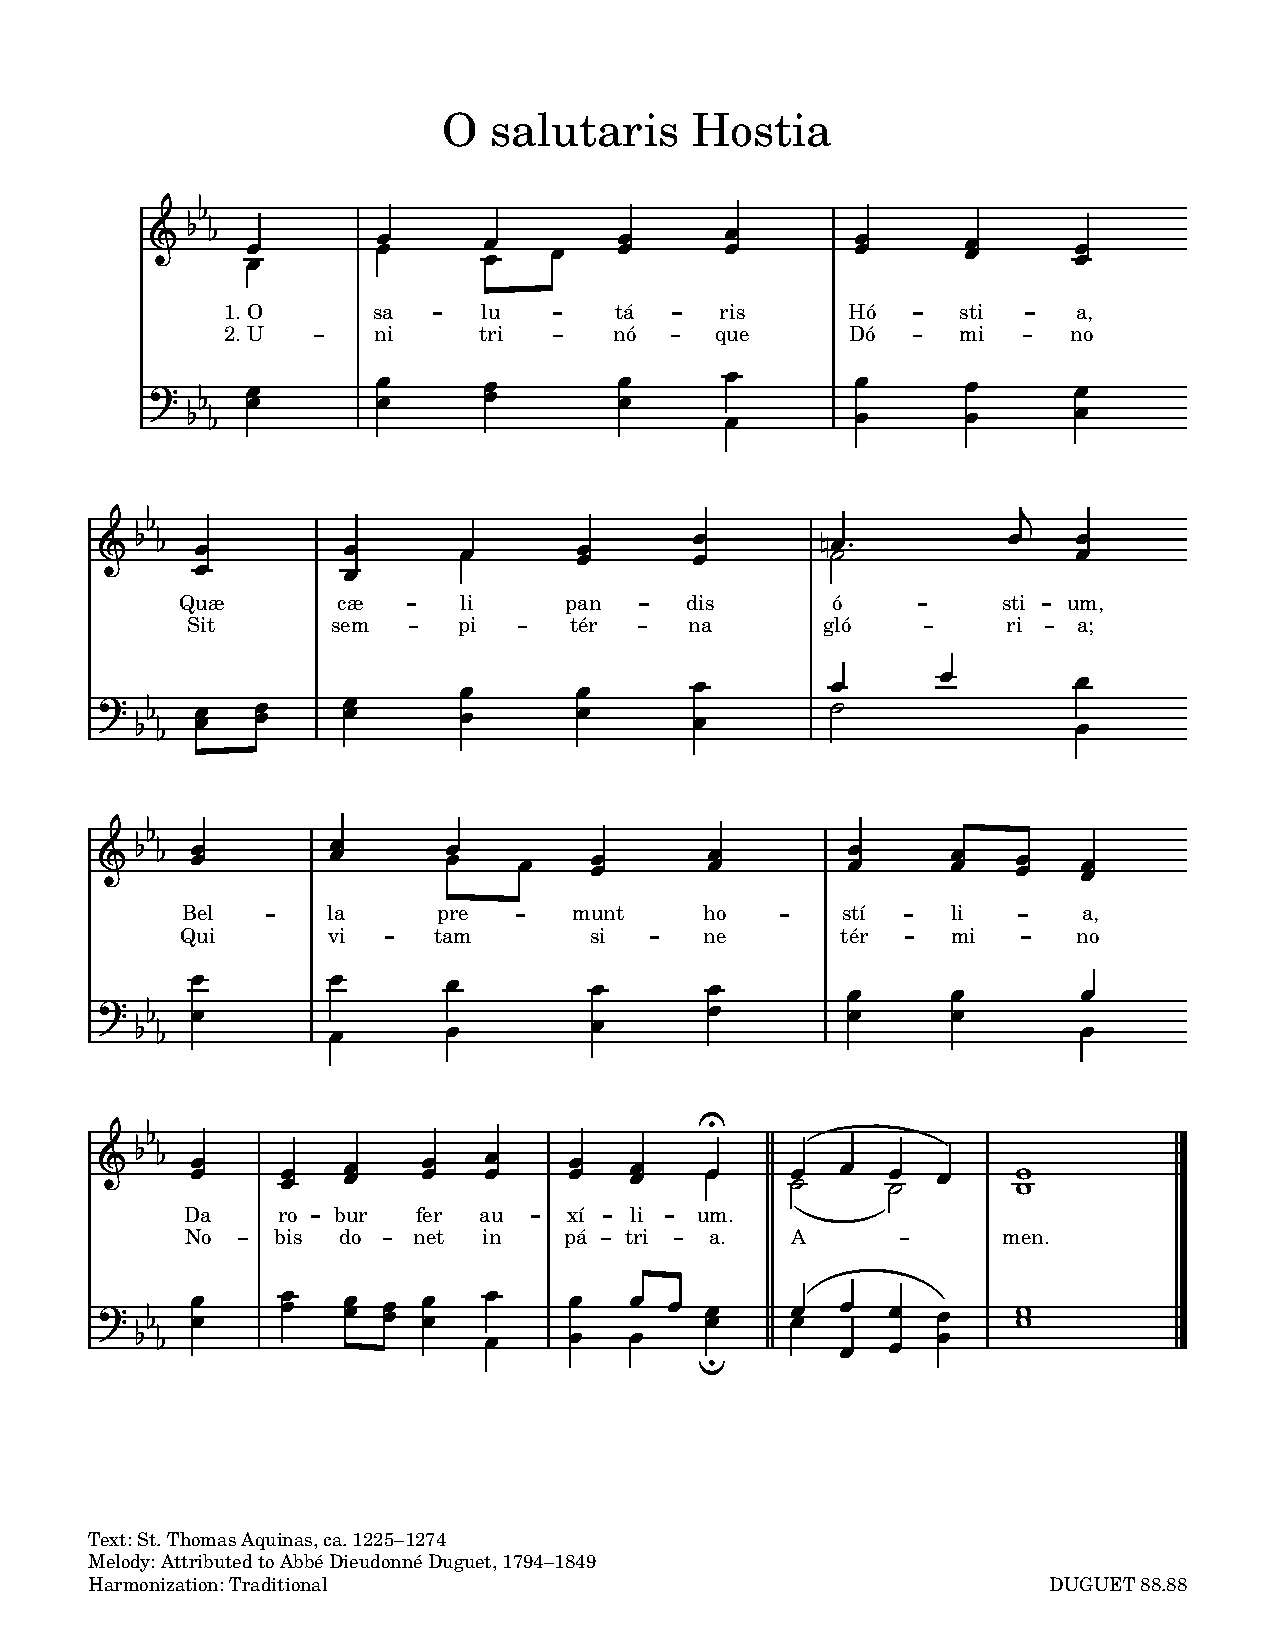
\includegraphics[width=123mm,height=193mm,keepaspectratio]{O_salutaris_Hostia_Duguet}
\newpage

\begin{otherlanguage}{english}{\centering{Prayer Before Benediction of the Most Holy Eucharist at Holy Hour}\par}

\rubrique{The priest says this prayer.}

O most sweet Jesus, who didst come into this world to enrich all souls with the life of Thy grace, and in order to preserve and foster that life within them, dost give Thyself day by day in the most adorable Sacrament of the Eucharist, as a saving remedy to heal their infirmities and a divine food to support their weakness: we humbly beseech Thee graciously to pour forth Thy Holy Spirit upon them all; so that, filled therewith, such as are defiled with deadly stain may return to Thee and recover the life of grace which they have forfeited by sin, and such as by the gift of Thy mercy already cleave to Thee may, as to each is given, approach every day Thy heavenly Banquet with true devotion. Strengthened thus, may they find herein an antidote to daily venial faults and a nourishing of the life of grace; that so being ever more and more cleansed, they may come to enjoy everlasting happiness in Heaven. ℟. Amen.

\rubrique{Then follows the prayer for the Sovereign Pontiff:}\kern 0.05em\footnote{\raggedright{Partialis indulgentia conceditur christifideli qui,…spiritu filialis devotionis, pro Summo Pontific aliquam prece legitime adprobatam pi recitaverit \textit{(e.g. Orémus pro Pontifice)} (Enchiridion Indulgentiarum, nº 25, 1º)}}

\noindent \vv Let us pray for our Pontiff, \textit{N.}

\noindent \rr The Lord preserve him, and give him life, | and make him blessèd upon the earth, | and deliver him up not up to the will of his enemies.

\noindent \vv Our Father…

\noindent \rr Give us this day…

\noindent \vv Hail Mary…

\noindent \rr Holy Mary…

\noindent \vv  Glory be…

\noindent \rr As it was…world without end. Amen.…

\rubrique{Priest:}

Almighty, everlasting God, have mercy upon Thy servant, \textit{N.,} our Sovereign Pontiff, and direct him, according to Thy clemency, into the way of everlasting salvation; that by Thy grace he may desire those things that are pleasing to Thee, and perform them with all his strength. ℟. Amen.

\rubrique{Then follows Benediction of the Most Blessed Sacrament, as usual.}


\end{otherlanguage}
%\begin{sloppypar}
% \begin{paracol}{2}
%  \setlength{\columnsep}{1.5em} %EB Garamond, Octavio Pardo; should define this so that there are no magic numbers
% \input{Pro_Papa_la}
%
%\switchcolumn
%
%\begin{otherlanguage}{english}


\noindent ℣. Let us pray for our Pontiff, \textit{N.}

\noindent ℟. The Lord preserve him, and give him life, | and make him blessèd upon the earth, | and deliver him up not up to the will of his enemies.

\noindent ℣. Our Father…

\noindent ℟. Give us this day…

\noindent ℣. Hail Mary…

\noindent ℟. Holy Mary…

\rubrique{Priest:}

Almighty, everlasting God, have mercy upon Thy servant, \textit{N.,}  our Sovereign Pontiff, and direct him, according to Thy clemency, into the way of everlasting salvation; that by Thy grace he may desire those things that are pleasing to Thee, and perform them with all his strength. ℟. Amen.

\rubrique{Then follows Benediction of the Most Blessed Sacrament, as usual.}


\end{otherlanguage}
%
%\end{paracol}
%\end{sloppypar}

\begin{otherlanguage}{english}{\centering{Prayer Before Benediction on Sundays at Holy Hour\kern 0.05em\footnote{\raggedright{Prayer adapted from Nicholas Stephen Cardinal Wiseman, Archbishop of\kern 0.25em West\-min\-ster (1802–1865).}}}\par}

{\centering{\rubrique{Used on all Sundays of the year, except on the second Sunday of each month.}}\par}

\rubrique{All kneel; the Priest begins:}

O Blessed Virgin Mary, (\textit{all join}) Mother of God | and our most gentle Queen and Mother, | look down in mercy upon us all | who greatly hope and trust in thee. | By thee it was that Jesus | our Savior and our Hope | was given unto the world; | and He has given thee to us | that we might hope still more.

Plead for us, thy children, | whom thou didst receive and accept | at the foot of the Cross, | O sorrowful Mother. | Intercede for our separated brethren, | that with us, | in the one true fold, | they may be united to the supreme Shepherd, | the Vicar of thy Son.

Pray for us all, dear Mother | that by faith | fruitful in good works, | we may all deserve to see and praise God, | together with thee, | in our heavenly home. Amen.

\rubrique{Then follows Benediction of the Most Blessed Sacrament of the Eucharist, in the usual way.}\end{otherlanguage}

%% Hard line break necessary to avoid the incorrect kerning in "of W"; the f and W touch, \kern is negative, and it or \thinspace change the interword space on the whole line. 

%kern 0.17em

\begin{otherlanguage}{english}
\rubrique{On the Second Sunday of each month, instead of the prayer \kern0.1em \normaltext{O Blessed Virgin Mary,} the following prayer is said, all kneeling.}

\rubrique{The priest says:}

O merciful God, let the glorious intercession of Thy saints assist us; above all, the most blessèd Virgin Mary, the Immaculate Mother of Thine only-begotten Son, and Thy holy apostles, Peter and Paul, through whose patronage we humbly commend this land. Be mindful of our fathers, Thy glorious bishop John Neumann; of Junípero and Damian, Thy priests. Remember our holy martyrs who shed their blood for Christ: Isaac, René and Jean. Remember those holy virgins and widows: Frances, Rose-Philippine, Katherine, Théodore, Marianne, Kateri, and Elizabeth Ann; and all those holy men and women who made this country illustrious by their glorious merits and virtues. Let not thy memory perish before Thee, O Lord, but let their supplication enter daily into Thy sight; and do Thou, who didst so often spare Thy sinful people for the sake of Abraham, Isaac, and Jacob, now, also moved by the prayers of our fathers, brothers, and sisters reigning with Thee, have mercy up on us, save Thy people and bless Thine inheritance; and suffer not those souls to perish which Thy Son hath redeemed with His own most Precious Blood: Who liveth and reignest with Thee, world without end. ℟. Amen.
\smallskip

Let us pray.

O most loving Lord Jesus, Who, when Thou wert hanging on the Cross, didst commend us all in the person of Thy disciple John to Thy most sweet Mother, that we might find in her our refuge, our solace and our hope; look graciously upon our beloved land, and on those who are bereaved of so powerful a patronage; that acknowledging the dignity of this Holy Virgin, they may honor and venerate her with all affection of devotion, and own her as Queen and Mother. May her sweet name be listed by little ones, and linger on the lips of the agèd and dying; and may it be invoked by the afflicted, and hymned by the joyful; that this Star of the Sea being their protection and their guide, all may come to the harbor of eternal salvation. Who liveth and reignest with Thee, world without end. ℟. Amen.\end{otherlanguage}

%\begin{multicols}{2}%
\begin{sloppypar}
 \begin{paracol}{2}
 \setlength{\columnsep}{1.5em} %EB Garamond, Octavio Pardo; should define this so that there are no magic numbers
Tantum ergo Sacramentum
Veneremur cernui:
Et antiquum documentum
Novo cedat ritui:
Præstet fides supplementum
Sensuum defectui.

Genitori, Genitoque
Laus et jubilatio,
Salus, honor, virtus quoque
Sit et benedictio:
Procedenti ab utroque
Compar sit laudatio. Amen.

℣. Panem de cælo præstitisti eis. \tpalleluia{}\footnote{Atque per octavam Corporis Christi. \textit{As well as throughout the octave of Corpus Christi.}}

℟. Omne dele\-ctaméntum in se habéntem. \tpalleluia{}
\par
Orémus.

Deus, qui nobis sub sacramento mirabili, passionis tuæ memoriam reliquisti: tribue, quæsumus, ita nos corporis et sanguinis tui sacra mysteria venerari, ut redemptionis tuæ fructum in nobis iugiter sentiamus. Qui vivis et regnas in sæcula sæculorum. ℟. Amen. 

%\columnbreak
\switchcolumn

%{\vulgata
\begin{otherlanguage}{english}Therefore so great a Sacrament
Let us fall down and worship,
and let the old law
give way to a new rite,
and let faith stand forward
to make good the defects of sense.

To the Father and the Son be praise and joy,
health, honour and virtue and blessing,
and to him proceeding from both
be equal praise.
Amen.

℣. Thou hast given them bread from heaven. (\textit{P.T.} Alleluia.)

℟. Having within it all sweetness. (\textit{P.T.} Alleluia.)

Let us pray.

O God, who in this wonderful Sacrament hast left us a memorial of Thy Passion: grant, we implore Thee, that we may so venerate the sacred mysteries of Thy Body and Blood, as always to be conscious of the fruit of Thy Redemption. Who livest and reignest forever and ever. ℟. Amen.\end{otherlanguage}
%}
%\end{multicols}
\end{paracol}
\end{sloppypar}

%\begin{center}
%During the week:
%\end{center}

{\centering{On Feasts.}\par}
\greannotation{3.}
\gregorioscore{hy--tantum_ergo_i--solesmes_1957}

{\centering{On Sundays.}\par}
\greannotation{5.}
\gregorioscore{hy--tantum_ergo_iii--solesmes_1957}

{\centering{During the week.}\par}
%\begin{center}
%During the week:
%\end{center}
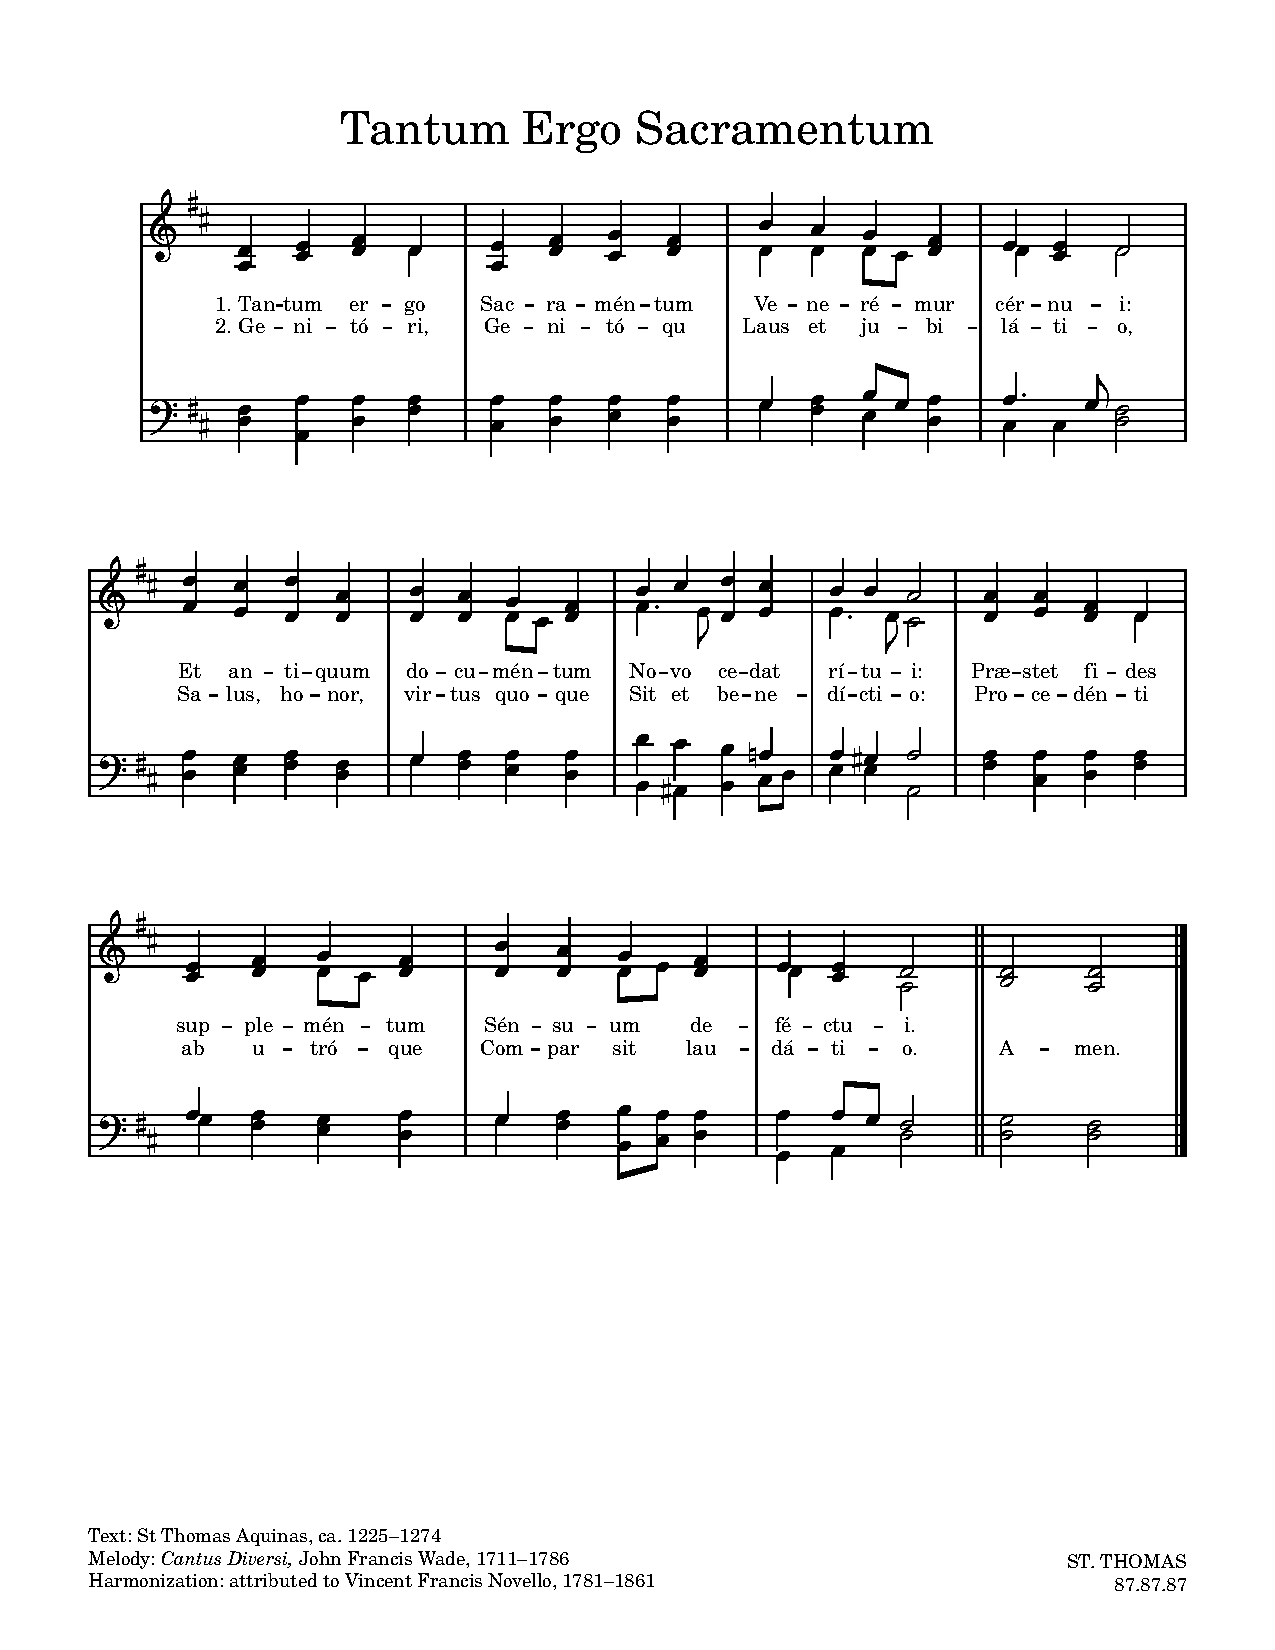
\includegraphics[width=123mm,height=193mm,keepaspectratio]{Tantum_Ergo_Sacramentum_Wade}

%\begin{center}
%On special occasions:
%\end{center}
{\centering{On special occasions.}\par}
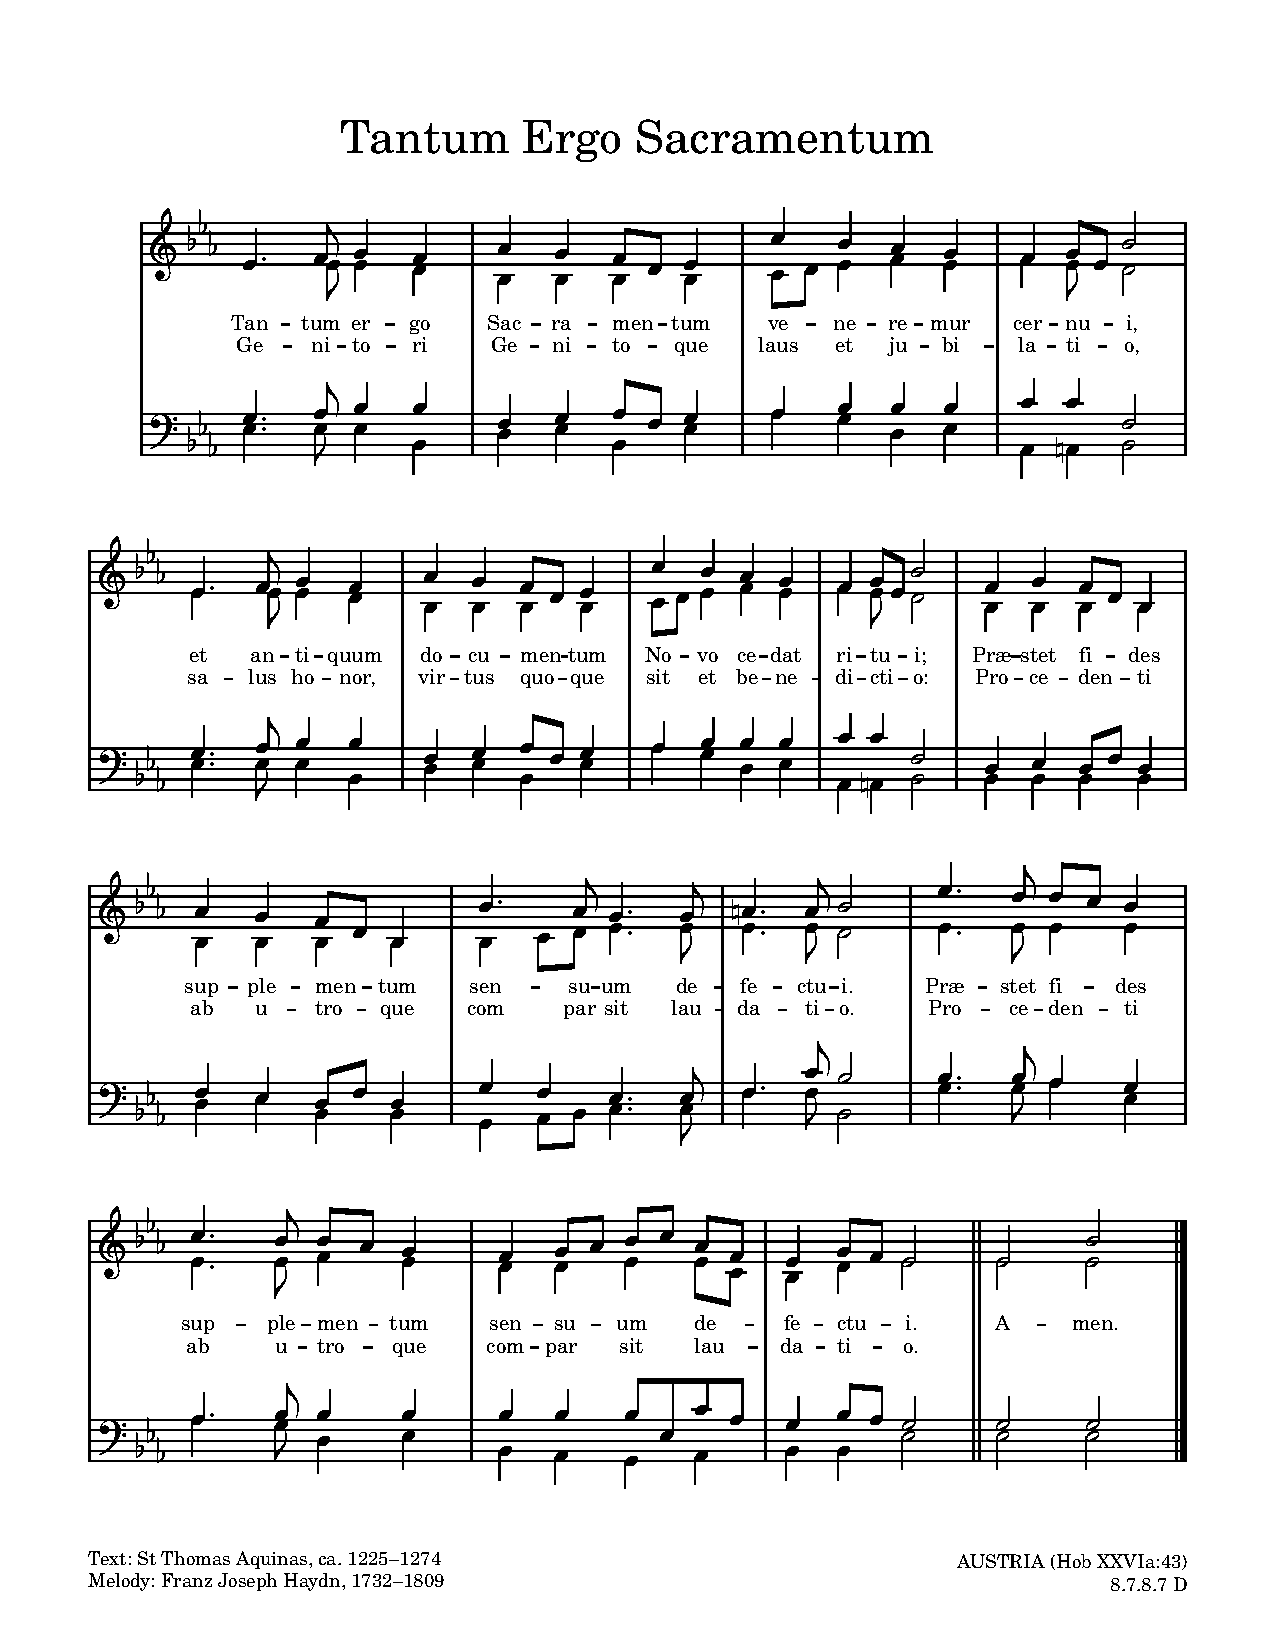
\includegraphics[width=123mm,height=193mm,keepaspectratio]{Tantum_Ergo_Sacramentum_Kaiserhymne}

\greannotation{5.}
\gregorioscore{ps_116_ad_Benedictionem}

\greannotation{5.}
\gregorioscore{va--adoremus_in_aeternum_i--solesmes_1957}

\greannotation{6.}
\gregorioscore{va--adoremus_ps_laudate_dominum_ii--solesmes}

\greannotation{1.}
\gregorioscore{va--cor_jesu--solesmes}

\greannotation{5.}
\gregorioscore{hy--adoro_te_devote--solesmes_1957}

\pstexte{Adoro_te_la}

%\greannotation{5.}
%\gregorioscore{hy--adoro_te_devote--solesmes} %%Full text

\greannotation{6.}
\gregorioscore{va--ave_verum--solesmes}

\greannotation{1.}
\gregorioscore{va--ave_maria_salutatio_angelica_solesmes_1961}
\smallskip
\begin{otherlanguage}{english}
Hail, Mary, full of grace,
the Lord is with thee.
Blessed art thou amongst women
and blessed is the fruit of thy womb, Jesus.
Holy Mary, Mother of God,
pray for us sinners,
now and at the hour of our death. 
Amen.
\end{otherlanguage}

\greannotation{7.}
\gregorioscore{an--sub_tuum_praesidium--solesmes}
\smallskip
\begin{otherlanguage}{english}Under thy protection we seek refuge, O Holy Mother of God;
In our neceessities, despise not our petitions,
but deliver us always from all dangers,
O Glorious and Blessed Virgin.
\end{otherlanguage}

\greannotation{6.}
\gregorioscore{se--inviolata--solesmes}
\smallskip
\begin{otherlanguage}{english}Inviolate, whole and chaste art thou, Mary:
Thou art the shining gate of heaven.
O kind mother, dearest to Christ,
receive our pious proclamations of praise.
To thee our devout hearts and mouths cry out:
may our souls and bodies be pure.
Through thy sweet sounding prayers
may thou grant us forgiveness forever.
O kindly one! O Queen! O Mary!
Thou alone didst remain inviolate.\end{otherlanguage}

\greannotation{1.}
\gregorioscore{va--oremus_pro_pontifice--solesmes}

\greannotation{7.}
\gregorioscore{an--tu_es_petrus_solesmes_1961}

\greannotation{℣.}
\gregorioscore{va--oremus_pro_antistite--solesmes_1957}

\greannotation{1.}
\gregorioscore{an--parce_domine--solesmes.1verse}

\end{document}


\enddocument